\section{Model problem}
    \label{model_problem}

    Let a solid delimited by the domain $\Omega$ in the current configuration, and by $\Omega_{0}$ in the initial configuration. It morphs through the action of volumetric forces in its inner body, and through the influence of contacts forces and imposed displacements at its surface.

    Let $\partial \Omega = \partial_N \Omega \oplus \partial_D \Omega$ with $\partial_N \Omega$ the part of $\partial \Omega$ subjected to contact forces (\textit{i.e.} to Neumann boundary conditions),
    and $\partial_N \Omega$ that to imposed displacements (\textit{i.e.} to Dirichlet boundary conditions).
    With similar notations, let $\partial \Omega_0 = \partial_D \Omega_0 \oplus \partial_N \Omega_0$.

    Let $\tensori{t}\subscript{\bm{N}}$ (resp. $\tensori{T}\subscript{\bm{N}}$) contact forces acting on $\partial_N \Omega$ (resp. $\partial_N \Omega_{0}$) and $\tensori{u}\subscript{\bm{D}}$ (resp. $\tensori{U}\subscript{\bm{D}}$) imposed displacements acting on $\partial_D \Omega$ (resp. $\partial_D \Omega_{0}$). Let $\tensori{f}\subscript{\bm{V}}$ (resp. $\tensori{F}\subscript{\bm{V}}$) volumetric forces acting in $\Omega$ (resp. $\Omega_{0}$).

    \begin{figure}[h!]
        \centering
        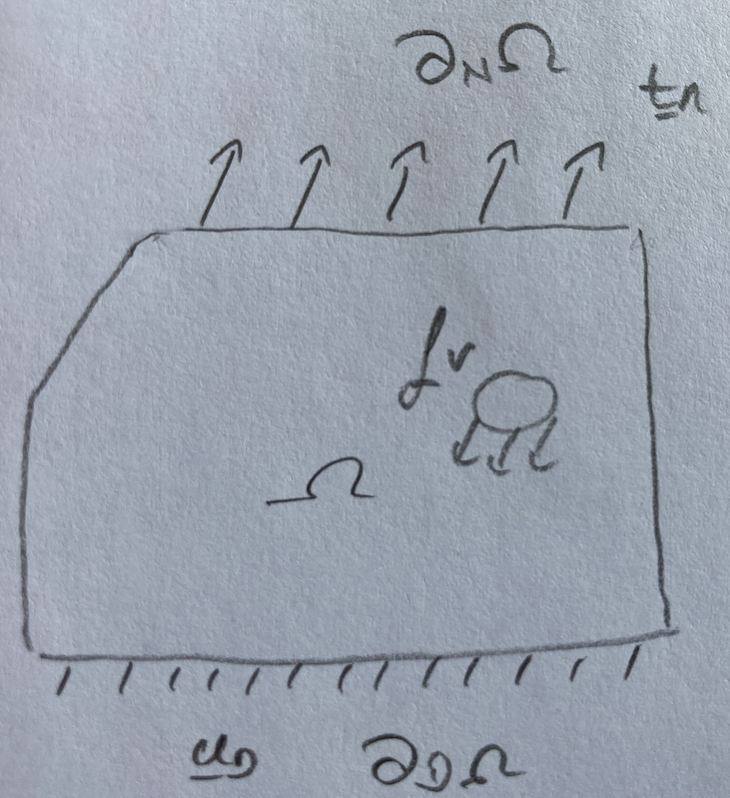
\includegraphics[width=7.cm]{img/fig_intro_0.png}
        \caption{The considered setting}
        \label{fig_intro_0}
    \end{figure}
    
    Let $\tensori{u}$ denote the displacement field and $\tensorii{\sigma}$ the stress tensor field in $\Omega$.

    The model problem in solid mechanics reads: find $\tensori{u}$ the displacement field in $\Omega$, such that
    \begin{equation}
        \label{eq_problem_0}
        \begin{aligned}
            & \nabla_x \cdot \tensorii{\sigma} = - \tensori{f}\subscript{\bm{V}}
            && \mbox{in $\Omega$}
            \\
            & \tensorii{\sigma} \cdot \tensori{n} = \tensori{t}\subscript{\bm{N}}
            && \mbox{on $\partial_N \Omega$}
            \\
            & \tensori{u} = \tensori{u} \subscript{\bm{D}}
            && \mbox{on $\partial_D \Omega$}
        \end{aligned}
    \end{equation}
    Performing an integration by part and multiplying by a test function $\tensori{u}$, one gets the weak form of \eqref{eq_problem_0}, \textit{i.e.} the principle of virtual works (PVW): find $\tensori{u}$ the displacement field in $\Omega$, such that, for all $\hat{\tensori{u}}$ kinematically admsissible :
    \begin{equation}
        \label{eq_problem_1}
        \begin{aligned}
            & \int_{\Omega} \nabla_x \hat{\tensori{u}}: \tensorii{\sigma}
            =
            \int_{\Omega} \hat{\tensori{u}} \cdot \tensori{f}\subscript{\bm{V}}
            +
            \int_{\partial_N \Omega} \hat{\tensori{u}} \cdot \tensori{t}\subscript{\bm{N}}
            &&
            \mbox{in $\Omega$}
            \\
            & \tensori{u} = \tensori{u} \subscript{\bm{D}}
            &&
            \mbox{on $\partial_D \Omega$}
        \end{aligned}
    \end{equation}
    In order to set the problem in the initial configuration, one needs to express it with respect to $\lighttensori{X} = \tensori{\Phi}\supscript{-1}(\lighttensori{x})$ the image in the initial configuration of a point $\lighttensori{x}$ in the reference configuration, and by the theorem of variable change under the integral sign, one has, for all $\hat{\tensori{u}}$ kinematically admsissible :
    \begin{equation}
        \label{eq_problem_2}
        \begin{aligned}
            & \int_{\Omega^0} \vert \det(\tensorii{F}) \vert \tensori{F}\supscript{-t} \nabla_X \hat{\tensori{u}}: \tensorii{\sigma}
            =
            \int_{\Omega^0} \hat{\tensori{u}} \cdot \vert \det(\tensorii{F}) \vert\supscript{-1} \tensori{f}\subscript{\bm{V}}
            +
            \int_{\partial_N \Omega^{0}} \hat{\tensori{u}} \cdot \vert \det(\tensorii{F}) \vert\supscript{-1} \tensorii{F}\supscript{-t} \tensori{t}\subscript{\bm{N}}
            &&
            \mbox{in $\Omega^{0}$}
            \\
            & \tensori{u} = \tensori{U}\subscript{\bm{D}}
            &&
            \mbox{on $\partial_D \Omega^{0}$}
        \end{aligned}
    \end{equation}
    Which becomes, defining $\tensorii{\Pi}\subscript{\bm{I}} = \vert \det(\tensorii{F}) \vert \tensorii{F}\supscript{-t} \tensorii{\sigma}$ the first Piola-Kirchoff stress tensor, $\tensori{F}\subscript{\bm{V}} = \vert \det(\tensorii{F}) \vert\supscript{-1} \tensori{f}\subscript{\bm{V}}$ the volumic forces and $\tensori{T}\subscript{\bm{N}} = \vert \det(\tensorii{F}) \vert\supscript{-1} \tensorii{F}\supscript{-t} \tensori{t}\subscript{\bm{N}}$ the contact forces in the initial confugurations :
    \begin{equation}
        \label{eq_problem_3}
        \begin{aligned}
            & \int_{\Omega^0} \nabla_X \hat{\tensori{u}}: \tensorii{\Pi}\subscript{\bm{I}}
            =
            \int_{\Omega^0} \hat{\tensori{u}} \cdot \tensori{F}\subscript{\bm{V}}
            +
            \int_{\partial_N \Omega^{0}} \hat{\tensori{u}} \cdot \tensori{T}\subscript{\bm{N}}
            &&
            \mbox{in $\Omega^{0}$}
            \\
            & \tensori{u} = \tensori{U}\subscript{\bm{D}}
            &&
            \mbox{on $\partial_D \Omega^{0}$}
        \end{aligned}
    \end{equation}

\newpage

\section{A mechanical introduction to the HHO method}

    \subsection{Geometrical and mechanical setting}
    \label{sec_HHO_0}

        The standard Finite Element (FE) method consists in seeking an approximation of the displacement field solving \eqref{eq_problem_0}.
        In order to do so, a mesh of the domain is introduced, to geomatrically descretize the problem, and the displacement field is approximated through shape functions, or, in other words, through nodal displacements.
        The displacement approximation is then a polynomial of order $1$ or $2$.
        In particular, the approximation of the displacement is continuous over the whole mesh, which is a natural assumption, since the actual displacement field in $\Omega$ is a continuum: in such a case, one speeks about conformal methods.

        Contrary to the FE method,
        the HHO methods assumes the discontuity of the displacement field across elements: this means that displacement jumps are allowed.
        Though, it is restricted, in the sense that elements are not totally independent from one another: indeed, one must consider that there exists an elastic interface around each element, linking them to their direct environement (\textit{i.e.} to their neighbours or to the boundary).
        Thus, let introduce $\Gamma$ the skeleton of the mesh, that is the set of all element interfaces $F$ in the mesh, be it with the boundary of the mesh, or between elements.
        Considering that the skeleton forms the structure to which the elastic interface is attachted to, one has introduced the geometric setting in which the HHO method fits into: elements (or cells), denoted by $T$, are directly disconected from one another, but they communicate through the elastic interface $\Upsilon$, which is fixed to the skeleton, \textit{i.e.} to the collection of all faces $F$. Moreover, let suppose all faces $F$ planar: hence, the interface $\Upsilon$ consists in a strip of homogeneous depth $l$ surrounding each element to its faces (see \figref{fig_intro_1}).

        \begin{figure}[h]
            \begin{minipage}{.5\textwidth}
                \centering
                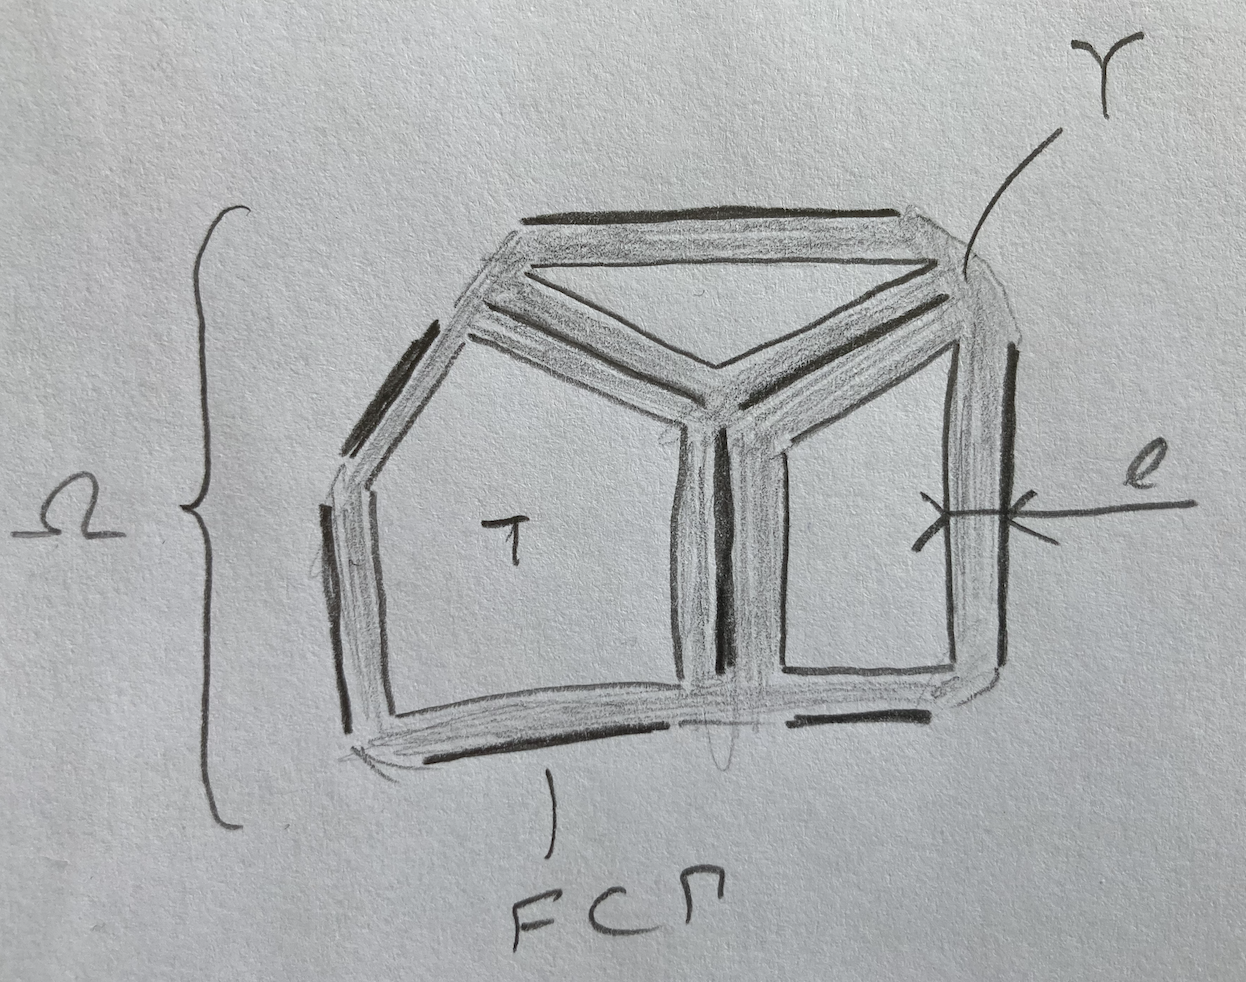
\includegraphics[width=5.cm]{img/fig_intro_1.png}
                \captionof{figure}{The mesh}
                \label{fig_intro_1}
            \end{minipage}%
            \begin{minipage}{.5\textwidth}
                \centering
                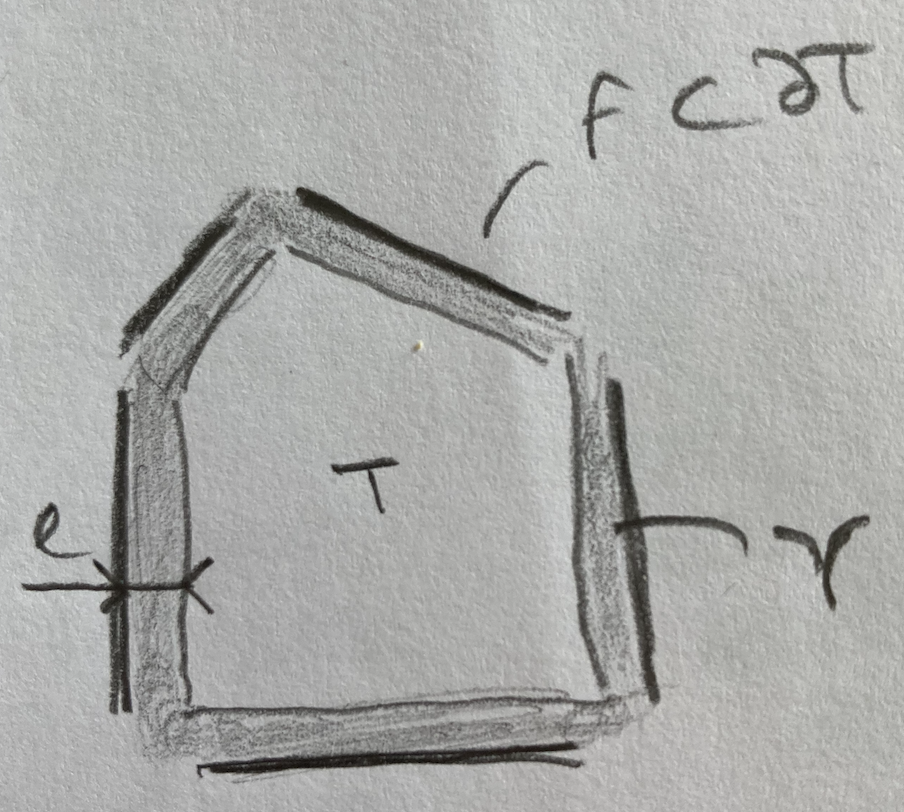
\includegraphics[width=5.cm]{img/fig_intro_2.png}
                \captionof{figure}{An element}
                \label{fig_intro_2}
            \end{minipage}%
        \end{figure}

        \paragraph{The considered setting}
        Let consider an elements $T$, linked to a boundary $\partial T$ composed of a collection of planar faces $F \subset \partial T$ through the elastic interface $\Upsilon$ (see \figref{fig_intro_2}).
        Let $\tensori{u}\subscript{\bm{T}}$ the displacement field in $T$, and $\tensori{u}\subscript{\bm{\partial T}}$ that on the skeleton: nothing apparently links $\tensori{u}\subscript{\bm{T}}$ to $\tensori{u}\subscript{\bm{\partial T}}$, except the elastic interface, whose contribution is evocated below.
        Let $\llbracket \tensori{u}\subscript{\bm{\partial T}} \rrbracket = \tensori{u}\subscript{\bm{\partial T}} - \tensori{u}\subscript{\bm{T}}$ the displacement jump between $T$ and $\partial T$.

        \paragraph{The interface $\Upsilon$ behaves like a linear elastic material}
        Let consider that $\Upsilon$ is made out of a linear elastic material with Young modulus $\beta$ and a zero Poisson coefficient, such that $\tensorii{\Pi}\subscript{\bm{I}} \vert_\Upsilon = \beta \ \tensorii{\varepsilon} \vert_{\Upsilon}$

        \paragraph{The interface $\Upsilon$ is thin with respect to $T$}
        Let consider that $\Upsilon$, with depth $l>0$, is thin with respect to the diameter of $T$. Hence, the behavior in $\Upsilon$ is approximated by that of a shell in three dimension or a beam in two dimension, with homogeneous deformation, such that both the gradient of the displacement and the deformation tensor take the simple forms
        \cite{1994_MICHEL_SUQUET_THEBAUD_UneModelisationDuRoleDesInterfacesDansLeComportementDesCompositesAMatriceMetallique}:
        \begin{equation}
            \label{eq_intro_0}
            \begin{aligned}
                \nabla \tensori{u} \vert_{\Upsilon}
                \approx
                \frac{\llbracket \tensori{u} \rrbracket}{l}
                \otimes
                \lighttensori{n}\subscript{\partial T}
                &&
                \text{and}
                &&
                \tensorii{\varepsilon} \vert_{\Upsilon}
                =
                \nabla^s \tensori{u} \vert_{\Upsilon}
                \approx
                \frac{1}{2}
                \big(
                    \frac{\llbracket \tensori{u} \rrbracket}{l}
                    \otimes
                    \lighttensori{n}\subscript{\partial T}
                    +
                    \lighttensori{n}\subscript{\partial T}
                    \otimes
                    \frac{\llbracket \tensori{u} \rrbracket}{l}
                \big)
                =
                \frac{\llbracket \tensori{u} \rrbracket}{l}
                \otimes^{s}
                \lighttensori{n}\subscript{\partial T}
            \end{aligned}
        \end{equation}

    \subsection{Inner traction force}

        Writing the equilibrium of the material in $T \cup \Upsilon$ and assuming that $\tensori{F}\subscript{\bm{V}}$ only acts in $T$ yields, for all $\hat{\tensori{u}}$ kinematically admissible :
        \begin{equation}
            \label{eq_inner_traction_force_0}
            \begin{aligned}
                % \text{(PVW)}\vert_{T \cup \Upsilon}
                \int_{T \cup \Upsilon} \nabla \hat{\tensori{u}}: \tensorii{\Pi}\subscript{\bm{I}}
                =
                \int_{T \cup \Upsilon} \hat{\tensori{u}} \cdot \tensori{F}\subscript{\bm{V}}
                &
                \iff
                \int_{T} \nabla \hat{\tensori{u}}: \tensorii{\Pi}\subscript{\bm{I}}
                +
                \int_{\Upsilon} \hat{\tensorii{\varepsilon}} \vert_{\Upsilon}: \tensorii{\Pi}\subscript{\bm{I}} \vert_{\Upsilon}
                =
                \int_{T} \hat{\tensori{u}} \cdot \tensori{F}\subscript{\bm{V}}
                \\
                &
                \iff
                \int_{T} \nabla \hat{\tensori{u}}: \tensorii{\Pi}\subscript{\bm{I}}
                +
                \int^{l}_{0}
                \int_{\partial T}
                ({\llbracket \hat{\tensori{u}} \rrbracket} {\otimes}^{s} \lighttensori{n}\subscript{\partial T}) :
                (\beta \ \frac{\llbracket \tensori{u} \rrbracket}{l} {\otimes}^{s} \lighttensori{n}\subscript{\partial T})
                =
                \int_{T} \hat{\tensori{u}} \cdot \tensori{F}\subscript{\bm{V}}
                \\
                &
                \iff
                \int_{T} \nabla \hat{\tensori{u}}: \tensorii{\Pi}\subscript{\bm{I}}
                +
                \int_{\partial T}
                \beta \ {\llbracket \hat{\tensori{u}} \rrbracket}
                \cdot
                {\llbracket \tensori{u} \rrbracket}
                =
                \int_{T} \hat{\tensori{u}} \cdot \tensori{F}\subscript{\bm{V}}
            \end{aligned}
        \end{equation}
        The volumic contribution in the expression of the equilibrium in $T \cup \Upsilon$ consists in the regular term in $T$, to which is added the contribution of the elastic interface $\Upsilon$, that writes as a traction force along the boundary of $T$ since the deformation in $\Upsilon$ is homogeneous.
        In the context of the HHO method, this traction force applied by the interface $\Upsilon$ is denoted the stabilization term, because it prevents the displacement in the cell $T$ to be completely disconected from that of its boundary $\partial T$: continuity of the displacement at the boundary of the cell is then expressed in a weaker sense.

    \subsection{Descrete gradient operator}
    
        Since the deformation is not homogeneous in $T \cup \Upsilon$ (there is no restriction about the transformation to be finite in $T$, whereas small strains are supposed in $\Upsilon$), one needs to consider the derivation process in a global way over $T \cup \Upsilon$.
        Hence, in place of the regular gradient operator $\nabla$, a global, mean gradient of the displacement, needs to be considered, that is taken to be the one that satisfies the projection of $\nabla \tensori{u}$ in $T \cup \Upsilon$ :
        \begin{equation}
            \begin{aligned}
                \int_{T \cup \Upsilon} \tensorii{\tau}: (\nabla \tensori{u} - \tensorii{G}\subscript{\bm{T}}) = 0
                \iff
                \int_{T \cup \Upsilon} \tensorii{\tau}: \tensorii{G}\subscript{\bm{T}}
                &
                =
                \int_{T \cup \Upsilon} \tensorii{\tau}: \nabla \tensori{u}
                \\
                &
                =
                \int_{T} \tensorii{\tau}: \nabla \tensori{u}\subscript{\bm{T}}
                +
                \int_{\Upsilon} \tensorii{\tau}: \nabla \tensori{u} \vert_{\Upsilon}
                \\
                &
                =
                \int_{T} \tensorii{\tau}: \nabla \tensori{u}\subscript{\bm{T}}
                +
                \int_{0}^{l}
                \int_{\partial T} \tensorii{\tau}: \frac{\llbracket \tensori{u} \rrbracket}{l} \otimes \lighttensori{n}\subscript{\partial T}
                \\
                &
                =
                \int_{T} \tensorii{\tau}: \nabla \tensori{u}\subscript{\bm{T}}
                +
                \int_{\partial T} \tensorii{\tau} \lighttensori{n}\subscript{\partial T} \cdot \llbracket \tensori{u} \rrbracket
            \end{aligned}
        \end{equation}
        In particular, $\tensorii{G}\subscript{\bm{T}}$ is a descrete gradient, defined only in $T$, that is enriched (with comparison to the regular displacement gradient $\nabla \tensori{u}$) with a term depending on the displacement jump across a cell and its boundary, through $\Upsilon$.

        Making now $l \rightarrow 0$ such that the volume of the interface $\Upsilon$ vanishes ($\Upsilon \rightarrow \emptyset$), there exists a discontuity at $\partial T$: both $\tensori{u}\subscript{\bm{T}}$, with value $\tensori{u}\subscript{\bm{T}}\vert_{\partial T}$ and $\tensori{u}\subscript{\bm{\partial T}}$ are defined at the boundary of $T$, but take different values.

        Finally, using the discrete gradient of the displacement field $\tensorii{G}\subscript{\bm{T}}$ in the PVW in place of the regular term $\nabla \tensori{u}$ yields, for all $\hat{\tensori{u}}$ kinematically admsissible :
        \begin{equation}
            \label{eq_final}
            \begin{aligned}
                \int_{T} \hat{\tensorii{G}}\subscript{\bm{T}}: \tensorii{\Pi}\subscript{\bm{I}}(\tensorii{G}\subscript{\bm{T}})
                +
                \sum_{F \in \partial T}
                \int_{F}
                % \frac{\beta}{h_F}
                \beta
                \llbracket \hat{\tensori{u}} \rrbracket
                \cdot
                \llbracket {\tensori{u}} \rrbracket
                =
                \int_{T} \hat{\tensori{u}}\subscript{\bm{T}} \cdot \tensori{F}\subscript{\bm{V}}
            \end{aligned}
        \end{equation}
        \eqref{eq_final} constitute the PVW as considered in the HHO method. In particular, taking the descrete gradient operator instead of the regular one is the key feature of the HHO method that proves to be robust in the incompressible case.